\subsection{Formato VGA}
\label{formatoVGA}

\begin{figure}[H]
	\centering
	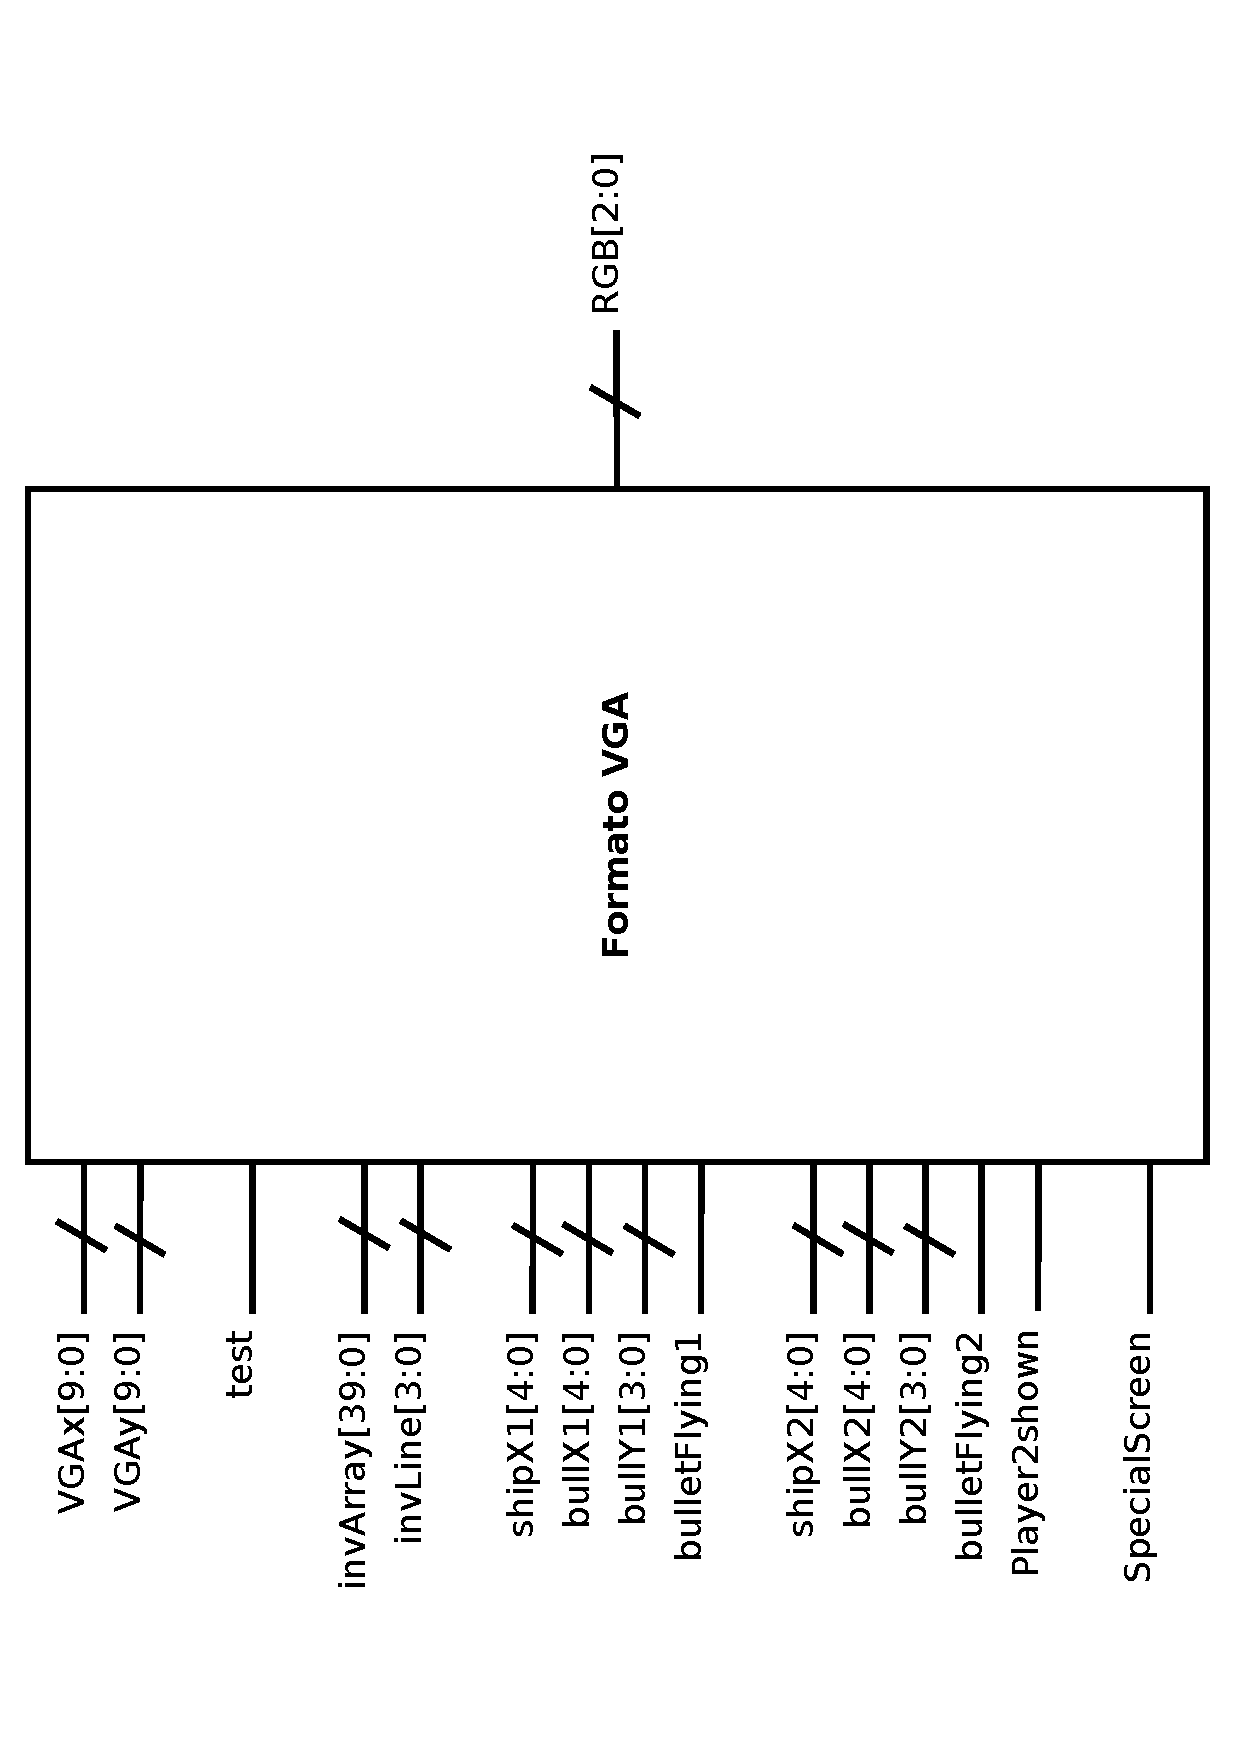
\includegraphics[width=0.4\textwidth, angle=-90] {formatoVGA_block.pdf}
	\caption{Interfaz del bloque Formato VGA}\label{fig:formatoVGA_block}
\end{figure}





El bloque \emph{Formato VGA} se encarga de traducir una serie de señales binarias procedentes de los invasores, naves y balas a figuras (\emph{sprites}) que mostrar en la pantalla.

\subsubsection*{Descripción del proceso}

Para facilitar esta tarea, la pantalla se divide en \emph{macropíxels}, celdas de 32 x 32 píxeles que contienen un sólo sprite. Así, el espacio de juego queda reducido a una matriz de 20 x 15 macropíxels. 

El proceso de dibujo de la pantalla pude resumirse de la siguiente manera:

\begin{enumerate}

\item El controlador VGA solicita la información RGB de un píxel.

\item \emph{Formato VGA} traduce la posición (x,y) a su correspodiente macropíxel.

\item Con la información procedente del resto de entidades, se selecciona qué elemento hay que mostrar en ese macropíxel.

\item Se accede a la matriz del sprite correspondiente, obteniedo el valor del píxel en concreto que se ha de dibujar.
\end{enumerate}

\subsubsection*{Codificación de la posición de los elementos}

La información posicional de los invasores, balas y naves se envía desde los diversos bloques a través de buses, que codifican la información de manera diferente:

\begin{itemize}
\item \textbf{Bala}: Cada una de las dos balas transmiten su posición en coordenadas de macropíxels, codificadas en dos buses de 5 y 4 bits respectivamente ($bullX_n$, $bullY_n$). La señal $bulletFlying_n$ indica si la bala de cada uno de los jugadores está activa.

\item \textbf{Nave:} Como la nave sólo puede moverse en la última línea de la pantalla, la señal $shipX_n$ basta para indicar su posición en el juego. Adicionalmente, la señal $player2shown$ indica si hay que mostrar la nave del jugador 2.

\item \textbf{Invasores:} La posición de cada uno de los invasores, así como su tipo, se codifica en las señales $invLine$ y $invArray$. $invLine$ define en qué linea se mueven los invasores, mientras que $invArray$ codifica el estado de los invasores (activo o abatido) y su nivel (más información en \hyperref[invaders]{Invasores}).

\end{itemize}